\documentclass[conference]{IEEEtran}
\usepackage{booktabs}
\usepackage{amsmath}
\usepackage{microtype}
\usepackage{float}
\usepackage{tikz}
\usepackage{hyperref}
\hypersetup{hidelinks}
\title{Auditing Multi-Task Graph Neural Networks for Political Tweet Classification}
\author{\IEEEauthorblockN{Viktor Najdovski}}

\begin{document}
\maketitle
\begin{abstract}
We compare graph convolution, neighborhood aggregation, and attention for two tasks on a collection of 7,053 political tweets: identifying one of 14 authors and predicting a binary misinformation \emph{pseudo-label}. An initial graph construction placed a direct edge between every tweet and its author account, making author identification partly an edge lookup. We remove those edges and account-profile features before evaluating three two-layer multi-task graph neural networks (GNNs) on a fixed tweet split. Across three initialization seeds, author macro-F1 ranges from 0.820 to 0.865 by architecture. GraphSAGE obtains 0.702 misinformation macro-F1, comparable to a text-only logistic regression baseline at 0.703. The audit changes the interpretation of the experiment: the graph supports author prediction, but these results do not establish an advantage over text alone for pseudo-label prediction.
\end{abstract}
\begin{IEEEkeywords}
graph neural networks, leakage audit, political tweets, weak supervision, misinformation
\end{IEEEkeywords}

\section{Introduction}
Graph neural networks combine a node's features with information from its neighbors. This is attractive for social-media analysis, where a tweet's text and the accounts that engage with it may both carry useful signals. It also creates an evaluation hazard: a graph can accidentally contain the answer to a prediction task. A model that recovers a directly encoded label can score well without learning a transferable relationship between language, interaction, and the target.

This study asks two questions. First, how much of author-identification performance survives after removing graph and feature shortcuts that directly expose the account? Second, does a GNN add anything to the prediction of automatically assigned misinformation labels beyond a text-only model? We compare three standard encoders---GCN~\cite{kipf2017}, GraphSAGE~\cite{hamilton2017}, and GAT~\cite{velickovic2018}---under one split and a shared multi-task objective. The central result is a change of interpretation: correcting the graph reduces author performance markedly, while the strongest GNN is essentially tied with a text-only baseline on the second target.

\section{Data and Labels}
The dataset contains 7,053 tweets from 14 Macedonian political accounts. After concatenating the 14 CSV files and deduplicating by tweet ID, the archive still contains 7,053 rows. The initial heterogeneous graph has 7,053 tweet nodes, 3,107 account nodes, and 97,364 directed edges. Tweet features consist of 256 TF--IDF text dimensions and five standardized numeric metadata fields: retweet, reply, and favorite counts, plus the author's follower and following counts. Account nodes have zero-valued features. Edges connect tweets to their authors and to accounts listed as retweeters; reverse edges permit bidirectional message passing.

The raw archive also shows important variation in available evidence. Of the 7,053 tweet texts, 150 (2.1\%) consist only of URLs, while 614 tweets (8.7\%) have no listed retweeters. The former offer little linguistic content to a text classifier, and the latter have no retweeter relation to supply graph context once the direct author edge is removed. These are properties of the raw data, not measured errors of any model; they identify cases where the two information sources may be weak.

The second target is derived from a multilingual zero-shot classifier, \texttt{joeddav/xlm-roberta-large-xnli}, using the candidate labels \texttt{valid}, \texttt{misleading}, and \texttt{invalid}. The observed counts are 5,303, 666, and 1,084, respectively. We merge the latter two into a positive binary class (1,750 tweets, or 24.8\%). These are model-generated labels, not independently verified fact-checks. In particular, the class names are candidate descriptions offered to the label generator; the experiment measures agreement with that procedure, not whether a political claim is true.

\section{Leakage Audit}
In the original graph, each tweet has a direct link to its author account. Since author identity is the first target, this is target leakage through topology. A two-layer GNN can also pass information from a tweet to its author account and back to other tweets by the same author. Randomly splitting tweet nodes does not remove that path: training and test tweets may share the same account node. Figure~\ref{fig:audit} shows the edge types considered in the audit.

Exactly 14,106 directed authorship edges---one in each direction for each tweet---are removed. An explicit post-filter check finds zero remaining direct tweet--author edges. We also zero the two tweet feature dimensions holding the author's follower and following counts, which could act as account fingerprints. Retweeter relations remain, giving a corrected graph with 83,258 directed edges. Because both edge and feature shortcuts are addressed, the before/after score change should be interpreted as a combined leakage correction, not an isolated estimate of the effect of one edge type.

\begin{figure}[t]
\centering
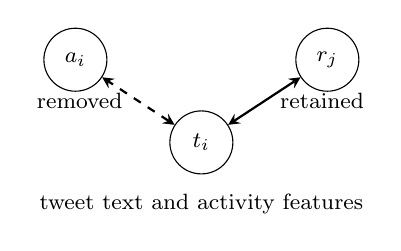
\begin{tikzpicture}[>=stealth, every node/.style={font=\footnotesize}]
  \node[draw,circle,minimum size=8mm] (tweet) at (0,0) {$t_i$};
  \node[draw,circle,minimum size=8mm] (author) at (-1.6,1.05) {$a_i$};
  \node[draw,circle,minimum size=8mm] (retweeter) at (1.6,1.05) {$r_j$};
  \draw[<->,dashed,thick] (tweet) -- node[left,xshift=-2pt] {removed} (author);
  \draw[<->,thick] (tweet) -- node[right,xshift=2pt] {retained} (retweeter);
  \node[align=center] at (0,-0.78) {tweet text and activity features};
\end{tikzpicture}
\caption{Graph audit for tweet $t_i$. The dashed authorship relation directly identifies the author target and is removed in both directions; retweeter relations remain.}
\label{fig:audit}
\end{figure}

\section{Experimental Setup}
Tweets are stratified by author into 4,513 training, 1,129 validation, and 1,411 test examples using a fixed split (seed 42). All models use the same tweet indices. The graph experiment is transductive: all nodes and non-target edges are visible, but only training tweet labels enter the loss. This evaluates classification of held-out tweets in a known network, not the arrival of new accounts or a future political event.

GNN input TF--IDF features were fitted on the full unlabeled tweet collection in the original preparation workflow; the text-only baseline fits its vocabulary on training tweets. Although no test labels are used in either vectorizer, this difference makes the feature-preparation protocols unequal and limits direct attribution of any small score difference to the graph.

Each encoder has two message-passing layers (96 hidden units), layer normalization, ReLU, dropout, and separate task heads. GAT uses two attention heads per layer. For a labeled tweet $i$, the training objective is
\begin{equation}
\mathcal{L}=\operatorname{CE}(\hat{a}_i,a_i)+
\operatorname{CE}_{(1,2)}(\hat{m}_i,m_i),
\end{equation}
where $a_i$ is the author class, $m_i$ is the binary pseudo-label, and $(1,2)$ denotes the negative and positive class weights. Each loss is averaged over training tweets before the task losses are added. The heads share the graph representation but not their final linear layers. This design makes author identification an auxiliary task for pseudo-label prediction, while also allowing competing gradients if the tasks favor different representations.

AdamW uses a learning rate of 0.008, weight decay of $10^{-4}$, and at most 35 epochs. Checkpoints are selected by mean \emph{post-update} validation macro-F1 across tasks, with early stopping after eight non-improving epochs. Evaluating validation predictions after the optimizer step matters: using cached training-pass logits would rank the newly updated checkpoint with predictions from the previous parameter state. Initializations use seeds 42, 43, and 44 on the fixed split.

For the pseudo-label task, we compare against majority-class prediction and class-balanced logistic regression on word unigram/bigram TF--IDF features (up to 30,000 terms). The vectorizer is fitted on the training tweets only. These baselines ask whether graph propagation improves upon a deliberately simple text predictor; they do not match the GNN's numeric metadata. Accuracy and macro-F1 are computed on the common test set. Macro-F1 gives equal weight to the two classes and therefore resists the misleading impression that could arise from predicting the 75\%-prevalent negative class alone. GNN scores are means $\pm$ sample standard deviations across three initialization seeds; baselines use one deterministic fit.

\section{Results}
Tables~\ref{tab:author} and~\ref{tab:pseudo} report the two tasks separately. They are interpreted as estimates under this fixed split and these generated labels, not as claims about factual accuracy in the wider political discourse.

\begin{table}[H]
\centering
\caption{Author identification after leakage removal (test macro-F1).}
\label{tab:author}
\begin{tabular}{lc}
\toprule
GNN encoder & Author macro-F1 \\
\midrule
GCN & $0.820\pm0.007$ \\
GraphSAGE & $0.857\pm0.016$ \\
GAT & $0.865\pm0.003$ \\
\bottomrule
\end{tabular}
\end{table}

\begin{table}[H]
\centering
\caption{Binary pseudo-label prediction (test macro-F1).}
\label{tab:pseudo}
\begin{tabular}{lc}
\toprule
Model & Pseudo-label macro-F1 \\
\midrule
Majority class & 0.428 \\
Text logistic regression & 0.703 \\
GCN & $0.688\pm0.003$ \\
GraphSAGE & $0.702\pm0.009$ \\
GAT & $0.669\pm0.004$ \\
\bottomrule
\end{tabular}
\end{table}

\subsection{Author Identification and the Leakage Diagnostic}
After the correction, GAT has the highest mean author macro-F1 (0.865), followed by GraphSAGE (0.857) and GCN (0.820). These scores show that author-related signal remains in tweet content, activity metadata, and retweeter neighborhoods; the direct authorship edge is not necessary to obtain above-chance classification. We do not know from these experiments which remaining source contributes most.

The original, unaudited graph produced author macro-F1 values of 0.957 (GCN), 0.989 (GraphSAGE), and 0.997 (GAT) in its reported run. Those near-perfect figures are retained only as a leakage diagnostic. They are not comparable as a controlled edge ablation: the corrected run also removes profile-count features and fixes validation checkpoint selection. Nevertheless, the original graph demonstrably contained the target relation, so its author scores should not be presented as valid generalization evidence. In the corrected seed-42 run, author macro-F1 is 0.827, 0.842, and 0.862 for GCN, GraphSAGE, and GAT, respectively.

\subsection{Pseudo-Label Prediction}
GraphSAGE has the highest mean GNN pseudo-label macro-F1 (0.702), followed by GCN (0.688) and GAT (0.669). The text-only logistic model obtains 0.703, while the majority baseline reaches just 0.428 despite 0.748 accuracy. Thus an accuracy-only comparison would conceal the majority model's complete failure to identify positive tweets. The GNN result does not establish a graph advantage on this pseudo-label task.

The confusion matrices help explain the near tie. On the seed-42 test set of 1,411 tweets, GraphSAGE produces $\left[\begin{smallmatrix}871&184\\139&217\end{smallmatrix}\right]$ and text logistic regression produces $\left[\begin{smallmatrix}827&228\\118&238\end{smallmatrix}\right]$, with rows ordered as true negative/positive and columns as predicted negative/positive. GraphSAGE makes 44 fewer false-positive predictions but 21 more false negatives. Its positive-class precision and recall are 0.541 and 0.610, versus 0.511 and 0.669 for logistic regression. GraphSAGE's higher accuracy (0.771 versus 0.755) therefore reflects a different operating trade-off, not uniformly better classification. The text model also has slightly higher balanced accuracy (0.726 versus 0.718).

\subsection{Variation Across Initializations}
The fixed-split three-seed comparison is small but prevents a single favorable initialization from becoming the whole result. GraphSAGE pseudo-label macro-F1 varies from 0.691 to 0.708, straddling the text baseline's 0.703. GAT is the most consistent author encoder in this set (0.862--0.868 across seeds), while GraphSAGE author scores span 0.842--0.873. These ranges are descriptive only: three seeds on one split do not provide a confidence interval for new datasets, accounts, or time periods.

\section{Discussion and Limitations}
The audit changes the scientific claim more than the architecture ranking. Under the original representation, a model could exploit an edge that encoded the author target. Under the corrected representation, author identification remains feasible but less striking. The comparison does not isolate the benefit of topology from text and metadata, nor does it prove that joint training is superior to a single-task model on the corrected graph. In particular, the older single-task runs used the unaudited graph and cannot serve as that control.

The pseudo-label task has a second interpretation problem: the target was itself inferred from tweet text. A text-only model can imitate that labeling procedure without detecting misinformation. The 150 URL-only tweets are a reminder that even the label generator may have limited semantic evidence for some examples. Without an independently annotated sample, agreement with generated labels cannot be converted into a claim about true or false political statements.

Other limits include one random, author-stratified split, possible overlap of related tweets across partitions, TF--IDF fitted on all unlabeled text for the GNN, and the absence of a corrected-graph feature-only neural baseline. A stronger next study would use verified labels, a temporal or account-held-out test, and an ablation that changes only graph edges while holding features, split, training, and validation procedures constant. It would also evaluate the 614 tweets without listed retweeters separately, since their corrected graph context is especially sparse.

\section{Conclusion}
This project compares three multi-task GNNs after auditing a direct authorship shortcut. GAT is strongest for corrected author identification, while GraphSAGE is strongest among GNNs for the generated misinformation label. The latter does not outperform a simple text-only baseline in macro-F1. The useful lesson is methodological: graph construction, target provenance, and a credible non-graph comparison determine what a high score can mean. With verified labels and stricter splits, the same framework could test whether political interaction structure provides information beyond tweet text.

\section*{Code Availability}
Source code and the Colab workflow are available in the \href{https://github.com/VikiShmiki/Political-Misinformation-Social-Networks}{GitHub repository}.

\begin{thebibliography}{9}
\bibitem{kipf2017} T. N. Kipf and M. Welling, ``Semi-Supervised Classification with Graph Convolutional Networks,'' \emph{ICLR}, 2017.
\bibitem{hamilton2017} W. L. Hamilton, R. Ying, and J. Leskovec, ``Inductive Representation Learning on Large Graphs,'' \emph{NeurIPS}, 2017.
\bibitem{velickovic2018} P. Veli\v{c}kovi\'c et al., ``Graph Attention Networks,'' \emph{ICLR}, 2018.
\end{thebibliography}
\end{document}
